\chapter{Discussion}\label{chapter:discussion}

Before discussing the outcomes of this work, we want to state a general remark. Our goal of training the network on the \ac{evc} dataset was not achievable, as we were not provided with the correct 3D object models. It is difficult to tell, how the networks would have performed on this dataset, as it appears to be more challenging in terms of image quality, occlusion, etc.

\section{Manual Annotation Process} \label{section:discussion_manual_annotation_process}

\begin{table}
\centering
    \begin{tabular}{|c||ccccc|} \hline
\diagbox{\# Object}{Image} & 0000.jpg & 0150.jpg & 0250.jpg & 0350.jpg & 0500.jpg \\ \hline\hline
\rowcolor{Gray}
01           &  0:53 & 2:29 & 0:20 & 0:03 & 0:06 \\ \hline
\end{tabular}
	\caption{The table shows the \textbf{absolute difference} between in minutes between correcting a pose using the controls of \ac{6dpat} and the new rotation feature. The comparison was only performed exemplary for object model 01 due to the limited time-frame of this work.} 
	\label{table:6dpat_improved_times}
\end{table}

The process of manually recovering poses using \ac{6dpat} comes along with some peculiarities, which we discuss here. By creating some annotations ourselves, we figured out that one of the bottlenecks of the program is the correction of poses after the initial position and rotation has been recovered from the clicked correspondences. The reason is that adjusting the values of the rotation and position by hand using the provided controls is slow and a try-and-error process. By trying to enter a higher rotational degree, the correct value was often surpassed. 

Despite the limited time of this work, we decided finally to improve the correction procedure by implementing functionality that allows easy rotation of the object model of a pose using the mouse. To make use of this new feature, the user has to select a pose to edit from the drop down list of poses and rotate the object model that is displayed by the pose editor (not pose viewer). This concept allowed the author to achieve the difference in times presented in Table \ref{table:6dpat_improved_times}. The discrepancy was computed only for the time needed to correct a pose, i.e. the time needed for clicking correspondences was not considered. This is not an empirical study and the superiority of the rotation method compared to manually editing the numbers needs to be proven for many images and datasets. But the provided times can serve as an indicator that directly rotating the object can be faster.

Next to \ac{6dpat}, we also faced some issues regarding the datasets themselves. Initially, a desired feature was to present another unannotated image after the user finishes annotating all poses in the current image. This is not feasible for multiple reasons. First of all, a user might still not be content with the poses. Selecting the next image programmatically could happen too early and thereby disrupt the annotation process of the user. The datasets can also have very distinct characteristics, which require the user to choose the next image manually. For a dataset like T-Less, many images have to be skipped due to their similarity. A network trained on one view on an object only, will likely predict inaccurate poses for a different view showing other characteristics of that object. The \ac{evc} dataset has less similar consecutive images.

The diversity of available datasets (see Section \ref{section:experiments_datasets} for a selection of datasets) is also the reason why the program does not provide functionality to initialize the next poses based on the ones in the last image. This feature would imply too many assumptions on the dataset and, in the worst case, cause more work for the user. 

While trying to annotate the images of the  dataset, it became clear that proper 3D models are crucial for successful annotation. To temporarily annotate the medical images, 3D surgical tools were downloaded from the internet as a replacement for the missing object models. But having a different shape and also missing the distinctive features of the real objects makes it very difficult to estimate the ground-truth pose. The influence of contradicting annotated poses during training of a network is not clear. The author of this work strongly recommends to obtain the correct 3D models before annotating the  images. The issue of the object models not fitting the segmentation mask can be seen in \fig \ref{fig:6dpat_sfb_segmentation}. \fig \ref{fig:6dpat_sfb_image} shows the actual image and the discrepancy between the object models and image pixels.

\begin{figure}
	\begin{subfigure}[t]{0.47\textwidth}
		\centering
    	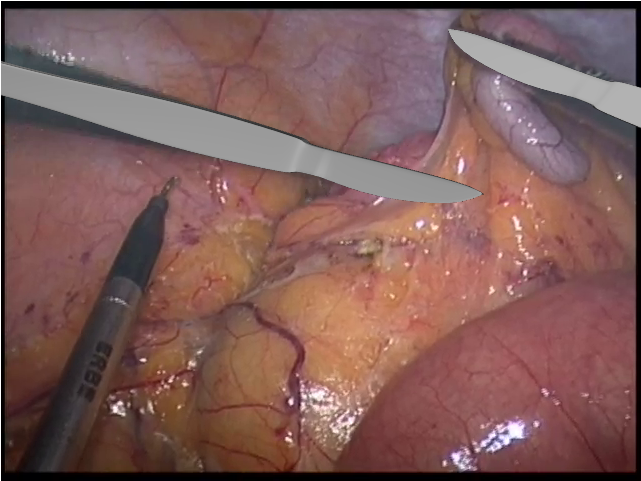
\includegraphics[width=\linewidth]{6dpat_sfb_image}
    	\caption{An image from the medical images dataset annotated using \ac{6dpat}. The correct rotation and translation are difficult to estimate without the correct 3D models.}
    	\label{fig:6dpat_sfb_image}
	\end{subfigure} 
	\hfill
	\begin{subfigure}[t]{0.47\textwidth}
		\centering
    	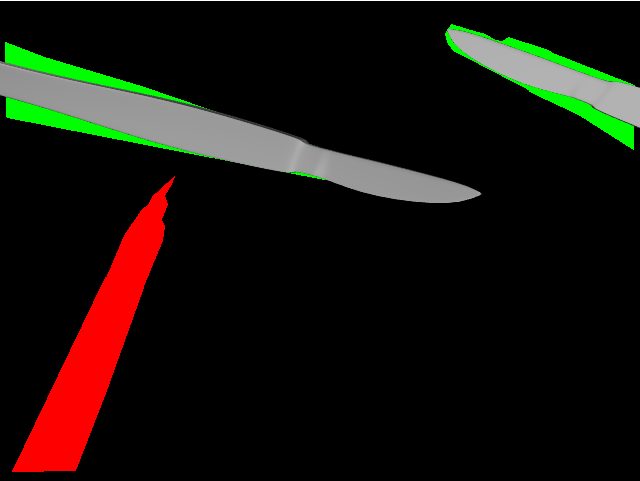
\includegraphics[width=\linewidth]{6dpat_sfb_segmentation}
    	\caption{The corresponding segmentation image. The discrepancy between the segmentation masks and the object model is the clearly visible green area.}
    	\label{fig:6dpat_sfb_segmentation}
	\end{subfigure} 
	\caption{Example annotations of images of the  dataset. The object model is taken from \cite{3d_scalpel_online}.}
	\label{fig:6dpat_sfb}
\end{figure} 

A general problem of any dataset can be seen in Appendix \ref{appendix:example_annotations} in form of the rotational error of manually annotated images. If the offset is similar in all recovered poses, this might not cause any trouble. If not, a network might be trained with contradicting object coordinates. There is no simple solution to this problem. Distinct characteristics of the object models could reduce this effect significantly, like the letters on the surgical tools in the  dataset or the notch of object model 01 of the T-Less dataset.

We think that \ac{6dpat} already resembles a program that can be used to annotate pose estimation datasets, efficiently and effectively already. Nevertheless, we provide improvement suggestions in Chapter \ref{chapter:future_work}.

\section{Semi-Automatic Annotation Process}

This section discusses the results of the experiments that we conducted using the network architectures of Chapter \ref{chapter:semi_automatic}. To this end, we analyze the outcomes in the order they appeared in Chapter \ref{chapter:experiments}. First, we want to make clear that some of the ways how we inferred conclusions underly some restrictions and are owed to the limited time of this work. An incremental training approach might have worked better for architectures 2 and 3, for example. We do not assume that this impacted the experiment results by a great extend but it has to be kept in mind when using the results for further research. We now state our interpretations of the training outcomes.

We conclude that the reduction of the receptive field-size without increasing the network's depth leads to a higher training and validation error. This can be seen in the discrepancy between the validation loss curves of architecture 1 and 3. Architecture 3 is as deep as architecture 1 (both 23 layers) but a reduced receptive field-size and a validation loss four times as high. Architecture 2 compensates the increased error related to the field-size by deeper design (35 layers). Architecture 5 achieves an error as low as architecture 1. Although its receptive field-size is smaller than that of architecture 2 (59 opposed to 67), we increased the number of layers to 50. Intuitively, by seeing less data (smaller receptive field-size) the network has to compensate this by being able to store more information somehow, thus the need for more layers.

It appears like all architectures memorize the training data quite well and achieve high pose inlier rates. But this does not hold for the metrics on the test set, although the test scenes are similar in terms of lightning conditions and image quality. We are unsure how the large drop of the performance of the networks on the test scene images compared to the training images came to exist.

Rad \etal report an average pose inlier rate of all objects visible in the test scene of 53.5 in \cite{bb8}. To the best of our knowledge, this is the only work providing an inlier rate on the T-Less dataset without using depth. This number is significantly higher than the accuracy we achieved. We expected even better results from our networks because the location of the object is already defined by the segmentation mask. Inspecting the metrics implies that the pose error is closely related to the error that captures the euclidean distance between the ground-truth and inferred translation vector. Since we predict poses on RGB-only images without depth information this is not too surprising. But this needs further investigation whether the $z$-coordinate is the one that causes the large distance errors.

Our initial assumption was that the networks are too deep and overfitted towards the data they were trained on. Despite the similar lightning conditions of the test images, we thought that the networks had taken in too many details of the training images. Since the validation images were taken from the pool of available training images, overfitting to the conditions of the training images can not be entirely prevented by such a validation set. But architecture 5 achieves the best pose inlier rate on the test set. Thus, it might be that the architectures are actually too shallow. Unfortunately, we were not able to explore this in depth in favor of examining the different training strategies.

The overall appearance of the validation losses of the incremental approaches is difficult to explain. The network seems to overfit but even if the training runs had been stopped in the valleys visible in \fig \ref{fig:experiments_online_sratch_90_10_validation_loss_arch1}, there would be a large gap compared to the training from scratch, still.

We cannot give a final statement why the incremental approach results in such an inferior validation loss. We assume that there is a way to improve this method so that it reaches the same level like the training from scratch. A reason for the inconsistent loss could be the trainable batch normalization. Training the network with 50 images first and then fixing the batch normalization weights could help decrease the validation loss when further training the network with datasets of 25 images. Although we expelled the SGD optimizer at the beginning of the experiments it could be that it is able to provide better results than Adam. We conclude this from the loss graphs of the incremental experiments, as the spiky curves could mean that Adam is not able to properly compute the learning rate. A very small rate set for SGD could yield different results. But for now, we have to recommend to train the network from scratch every time the user has manually annotated another batch of images.

The active training scheme on the other hand did provide better validation losses, i.e. selecting the images with the smallest IoU with the ground-truth segmentation masks reduced the validation loss significantly. This way, the validation loss of the experiment of training the network with 100 images from scratch was reached. Training with 50 of these images first and then incrementally training the network with the remaining 50 images resulted in a high validation loss. The results on the test set imply that this does not reliably mean that the network performs better in general. This is a sever issue and needs further investigation before drawing any conclusions.

We still suggest using a network together with \ac{6dpat}. We think that an unannotated dataset like \ac{evc} can still profit from the approximate locations predicted by a neural network. Although poses on the test sets seem to be inaccurate, the poses can be accurate when the network is trained on very similar images. For example, training architecture 1 with 250 images yields 78\% inlier on the validation set. Since we extracted validation images at regular intervals which ensures an even distribution, we conclude that the precision of the network is similar or only slightly below for the rest of the images. This means that predicted poses on images that the network was not trained with probably only need slight corrections. The fully annotated dataset can then be used to train a new network design that performs better on the test images.